\documentclass[12pt,a4paper]{report}
\usepackage[T2A]{fontenc}
\usepackage[utf8]{inputenc}
\usepackage[russian]{babel}
\usepackage{graphicx, setspace, amsmath}
\usepackage{minted}

\usepackage[
top = 1.25cm, 
bottom = 2.0cm]{geometry}

\begin{document}
\begin{titlepage} 
	\centering
    % HEADER
	{
        \scshape
        Федеральное государственное автономное образовательное учреждение высшего образования
        \par
        \textbf{«Научно-образовательная корпорация ИТМО»}
        \par
        \vspace*{1cm}
        Факультет Программной Инженерии и Компьютерной Техники
        \par
    }
    % LOGO
    \vspace*{0.6cm}
    
\includegraphics[width=\textwidth]{logo.png}
    % LAB INFO
    {
        \Large
        \textbf{Лабораторная работа по\\<<Тестированию программного обеспечения>> №1}
        \par
        \normalsize
        \vspace*{0.75cm}
        \textbf{Вариант 368849}
        \par
    }
    \vfill
    % СREDITS
    \hfill\begin{minipage}{\dimexpr\textwidth-7.8cm}
        \textbf{Выполнил:}\par
        Степанов Арсений Алексеевич\par
        \vspace*{0.15cm}
        \textbf{Группа:}\par
        P3318\par
        \vspace*{0.15cm}
        \textbf{Преподаватель:}\par
        Егошин Алексей Васильевич\par
    \end{minipage}
    \vfill
    Санкт-Петербург, \the\year{}г.
\end{titlepage}  
\section*{Задание}
\begin{enumerate}
    \item Для функции $\sec(x)$ провести модульное тестирование разложения функции в степенной ряд. Выбрать достаточное тестовое покрытие.
    \item Провести модульное тестирование сортировки пузырьком. Для этого выбрать характерные точки внутри алгоритма, и для предложенных самостоятельно наборов исходных данных записать последовательность попадания в характерные точки. Сравнить последовательность попадания с эталонной.
    \item Сформировать доменную модель для заданного текста.  Разработать тестовое покрытие для данной доменной модели:
\end{enumerate}
Артур неожиданно почувствовал, как на его бесплотной голове зашевелились волосы, когда он начал медленно, но неуклонно двигаться к пульту, но это был всего лишь, как он тут же догадался, наезд камеры при съемке.
\newpage
\section*{Выполнение}
\subsection*{Реализация и тестирование функции секанса}
Функция секанса выглядит как $\sec(x)=\frac{1}{\cos(x)}$, соответственно используя ряд Маклорена можно расчитать значение функции $\cos(x)$ в окрестностях нуля и на основе этого вычислить значение секанса
$$
\cos x = \sum_{n=0} (-1)^n\frac{x^{2n}}{(2n)!}
\qquad
\sec x=\frac{1}{\cos x}
$$
Реализация функции секанса:
\begin{minted}[fontsize=\small, frame=lines, linenos]{cpp}
using defaults::DEFAULT_TERMS;
using precision::Eps;

template <typename T>
constexpr T abs(T x) {
    return x < T{0} ? -x : x;
}

template <typename T>
requires std::floating_point<T>
constexpr T cos(T x, size_t terms = DEFAULT_TERMS<T>) {
    T result{1.0};
    T current_x{1.0};
    int16_t sign = 1;
    T fac = 1;

    for (size_t it = 1; it < terms; ++it) {
        current_x *= x * x;
        fac *= (2 * it - 1) * (2 * it);
        sign *= -1;
        if (std::isnan(current_x) || std::isnan(fac) || std::isnan(result + sign * current_x / fac))
            break;
        result += sign * current_x / fac;
    }

    return result;
}

template <typename T>
requires std::integral<T>
constexpr float cos(T x, size_t terms = DEFAULT_TERMS<T>) {
    return cos(static_cast<float>(x), terms);
}

template <typename T>
requires std::floating_point<T>
constexpr T sec(T x, size_t terms = DEFAULT_TERMS<T>) {
    if (std::isinf(x) || std::isnan(x)) {
        return std::numeric_limits<T>::quiet_NaN();
    }

    if (x < 0) {
        x = -x;
    }

    constexpr T PI = std::numbers::pi_v<T>;
    auto pi_shift = static_cast<int32_t>(x / (PI * 2));
    x += -pi_shift * 2 * PI;

    if (abs(x - PI / 2) < Eps<T>::VALUE || abs(x - 3 * PI / 2) < Eps<T>::VALUE) {
        return std::numeric_limits<T>::quiet_NaN();
    }
    return 1 / cos(x, terms);
}

template <typename T>
requires std::integral<T>
constexpr float sec(T x, size_t terms = DEFAULT_TERMS<T>) {
    return sec(static_cast<float>(x), terms);
}
\end{minted}
Для проверки работоспособности функции секанса я решил использовать разбиение на
классы эквивалентности, функция секанса является периодической с интервалом в $2\pi$, имеет точки разрыва
в $x=\frac{\pi}{2}+\pi k$
и имеет вид:\\
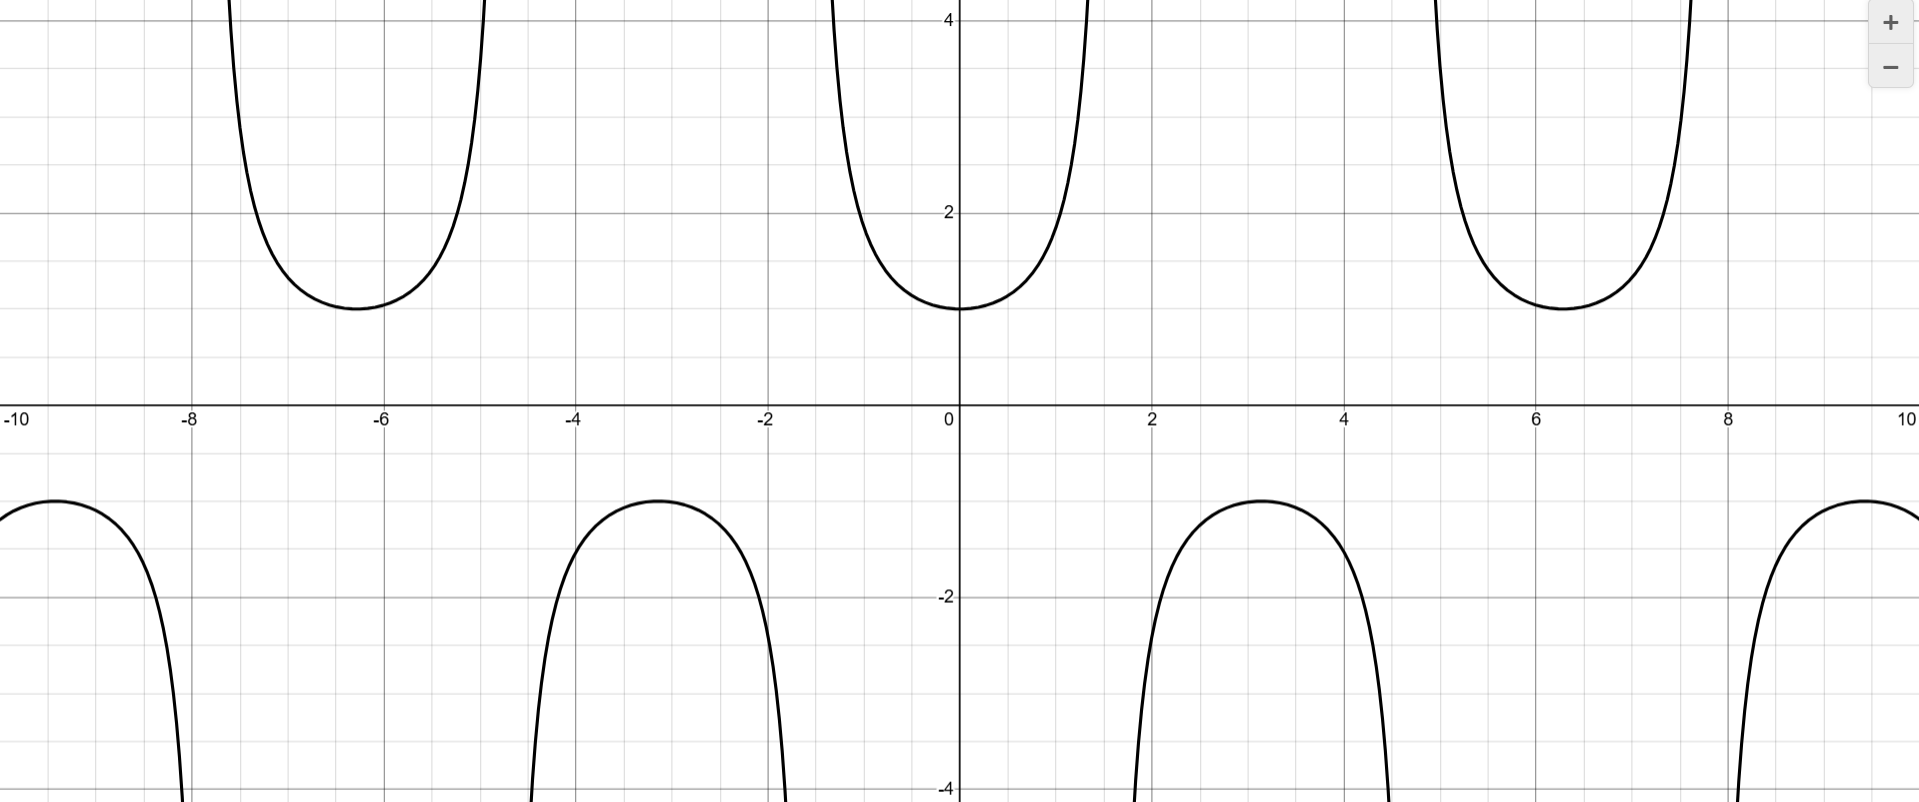
\includegraphics[width=\textwidth]{image.png}\\
На основе этого я выделил следующие классы для тестирования:
\begin{itemize}
    \item Значения функции в точках разрыва $x=\dfrac{\pi}{2}+\pi k$
    \item Значения функции в точках экстремума $x=\pi k$
    \item Значения функции в интервале возрастания $x\in(2\pi k, \dfrac{\pi}{2} + 2\pi k)$
    \item Значения функции в интервале убывания $x\in(\dfrac{\pi}{2} + 2\pi k, \pi + 2\pi k)$
    \item Значения функции в интервале возрастания $x\in(\pi + 2\pi k, \dfrac{3\pi}{2} + 2\pi k)$
    \item Значения функции в интервале убывания $x\in(\dfrac{3\pi}{2} + 2\pi k, 2\pi + 2\pi k)$
    \item Значения функции при положительном и отрицательном аргументах
\end{itemize}
А так же дополнительные проверки краевых случаев и специфики работы с типами с плавающей запятой:
\begin{itemize}
    \item Проверка что при подаче на вход значений NaN, функция так же вернёт NaN
    \item Проверка что при использовании типа float сохраняется точность как минимум до 3-ёх знаков после запятой
    \item Проверка что при использовании типа double сохраняется точность как минимум до 5-ти знаков после запятой
    \item Проверка что при использовании типа long double сохраняется точность как минимум до 7-ми знаков после запятой
\end{itemize}
Реализация тестов:
\begin{minted}[fontsize=\small, frame=lines, linenos]{cpp}
#include <gtest/gtest.h>
#include <cmath>
#include <numbers>
#include <type_traits>

#include <maths/maths.hpp>
#include <maths/defaults.hpp>

using arms::maths::sec;
using arms::maths::precision::Eps;

template <typename T>
class SecTest : public testing::Test {};

using FloatingPointTypes = testing::Types<float, double, long double>;
TYPED_TEST_SUITE(SecTest, FloatingPointTypes);

TYPED_TEST(SecTest, TestPointsOfDiscontinuity) {
    using T = TypeParam;
    constexpr auto PI = std::numbers::pi_v<T>;

    EXPECT_TRUE(std::isnan(sec(-PI / 2)));
    EXPECT_TRUE(std::isnan(sec(PI / 2)));
    EXPECT_TRUE(std::isnan(sec(3 * PI / 2)));
}

TYPED_TEST(SecTest, TestDiscontinuityNeighborhoodRegion) {
    using T = TypeParam;
    constexpr auto PI = std::numbers::pi_v<T>;

    EXPECT_FALSE(std::isnan(sec(-PI / 2 - Eps<T>::VALUE)));
    EXPECT_FALSE(std::isnan(sec(-PI / 2 + Eps<T>::VALUE)));
    EXPECT_FALSE(std::isnan(sec(PI / 2 - Eps<T>::VALUE)));
    EXPECT_FALSE(std::isnan(sec(PI / 2 + Eps<T>::VALUE)));
}

TYPED_TEST(SecTest, TestInfinity) {
    using T = TypeParam;
    constexpr auto INF = std::numeric_limits<T>::infinity();

    EXPECT_TRUE(std::isnan(sec(INF)));
    EXPECT_TRUE(std::isnan(sec(-INF)));
}

TYPED_TEST(SecTest, TestZero) {
    using T = TypeParam;

    EXPECT_NEAR(sec(static_cast<T>(0.0)), static_cast<T>(1.0), Eps<T>::VALUE);
}

TYPED_TEST(SecTest, TestRange1) {
    using T = TypeParam;

    EXPECT_NEAR(sec(static_cast<T>(0.228)), static_cast<T>(1.02656714459), Eps<T>::VALUE);
    EXPECT_NEAR(sec(static_cast<T>(0.322)), static_cast<T>(1.05418023973), Eps<T>::VALUE);
    EXPECT_NEAR(sec(static_cast<T>(1.337)), static_cast<T>(4.31644314933), Eps<T>::VALUE);
}

TYPED_TEST(SecTest, TestRange2) {
    using T = TypeParam;

    EXPECT_NEAR(sec(static_cast<T>(1.7)), static_cast<T>(-7.76129399605), Eps<T>::VALUE);
    EXPECT_NEAR(sec(static_cast<T>(1.812)), static_cast<T>(-4.18634900555), Eps<T>::VALUE);
    EXPECT_NEAR(sec(static_cast<T>(2.28)), static_cast<T>(-1.53555659487), Eps<T>::VALUE);
}

TYPED_TEST(SecTest, TestRange3) {
    using T = TypeParam;

    EXPECT_NEAR(sec(static_cast<T>(3.22)), static_cast<T>(-1.00308174955), Eps<T>::VALUE);
    EXPECT_NEAR(sec(static_cast<T>(4.2)), static_cast<T>(-2.03973060149), Eps<T>::VALUE);
    EXPECT_NEAR(sec(static_cast<T>(4.6)), static_cast<T>(-8.91642861136), Eps<T>::VALUE);
}

TYPED_TEST(SecTest, TestRange4) {
    using T = TypeParam;

    EXPECT_NEAR(sec(static_cast<T>(4.88)), static_cast<T>(5.99422183928), Eps<T>::VALUE);
    EXPECT_NEAR(sec(static_cast<T>(5)), static_cast<T>(3.52532008582), Eps<T>::VALUE);
    EXPECT_NEAR(sec(static_cast<T>(5.13)), static_cast<T>(2.46561733623), Eps<T>::VALUE);
}

TYPED_TEST(SecTest, TestExtremum) {
    using T = TypeParam;
    constexpr auto PI = std::numbers::pi_v<T>;

    EXPECT_NEAR(sec(-PI), -1.0, Eps<T>::VALUE);
    EXPECT_NEAR(sec<T>(0.0), 1.0, Eps<T>::VALUE);
    EXPECT_NEAR(sec(PI), -1.0, Eps<T>::VALUE);
}

TYPED_TEST(SecTest, TestIntervals) {
    using T = TypeParam;
    constexpr T INITIAL = 0.1459;
    constexpr auto PI = std::numbers::pi_v<T>;
    constexpr auto INTERVAL = 2 * PI;

    EXPECT_NEAR(sec(INITIAL), sec(INITIAL - INTERVAL * 30), Eps<T>::VALUE);
    EXPECT_NEAR(sec(INITIAL), sec(INITIAL - INTERVAL * 20), Eps<T>::VALUE);
    EXPECT_NEAR(sec(INITIAL), sec(INITIAL - INTERVAL * 10), Eps<T>::VALUE);
    EXPECT_NEAR(sec(INITIAL), sec(INITIAL + INTERVAL * 10), Eps<T>::VALUE);
    EXPECT_NEAR(sec(INITIAL), sec(INITIAL + INTERVAL * 20), Eps<T>::VALUE);
    EXPECT_NEAR(sec(INITIAL), sec(INITIAL + INTERVAL * 30), Eps<T>::VALUE);
}
\end{minted}
\subsection*{Реализация и тестирование функции сортировки пузырьком}
Реализация сортировки пузырьком:
\begin{minted}[fontsize=\small, frame=lines, linenos]{cpp}
template <std::random_access_iterator RandomIt, class Compare>
requires std::indirect_strict_weak_order<Compare, RandomIt>

constexpr void bubble_sort(RandomIt first, RandomIt last, Compare comp) {
    if (first == last) {
        return;
    }

    for (auto unsorted_end = last; unsorted_end != first; --unsorted_end) {
        bool swapped = false;
        for (auto it = first; (it + 1) < unsorted_end; ++it) {
            auto next = it + 1;
            if (std::invoke(comp, *next, *it)) {
                std::iter_swap(it, next);
                swapped = true;
            }
        }

        if (!swapped) {
            return;
        }
    }
}

template <std::random_access_iterator RandomIt>
constexpr void bubble_sort(RandomIt first, RandomIt last) {
    bubble_sort(first, last, std::less<>{});
}
\end{minted}
Для проверки работоспособности алгоритма сортировки были выделены некоторые краевые случаи и проверка поведения алгоритма:
\begin{itemize}
    \item Проверка того что алгоритм правильно сортриует переданный контейнер
    \item Проверка того что алгоритм сортирует по возрастанию по-умолчанию
    \item Проверка того что алгоритм корректно работает с компараторами
    \item Проверка того что алгоритм корректно работает с отрицательными числами и дублирующимися значениями
    \item Проверка того что алгоритм корректно работает на пустом контейнере
    \item Проверка того что алгоритм корректно работает на контейнере с одним элементом
\end{itemize}
Реализация тестирования:
\begin{minted}[fontsize=\small, frame=lines, linenos]{cpp}
TEST(BubbleSortTest, SortsAscendingByDefault) {
    std::vector<int> values{5, 1, 4, 2, 8};
    arms::sorting::bubble_sort(values.begin(), values.end());

    EXPECT_EQ(values, (std::vector<int>{1, 2, 4, 5, 8}));
}

TEST(BubbleSortTest, SortsDescendingWithComparator) {
    std::vector<int> values{5, 1, 4, 2, 8};
    arms::sorting::bubble_sort(values.begin(), values.end(), std::greater<>{});

    EXPECT_EQ(values, (std::vector<int>{8, 5, 4, 2, 1}));
}

TEST(BubbleSortTest, HandlesDuplicatesAndNegatives) {
    std::vector<int> values{3, -1, 3, 2, -1, 0};
    arms::sorting::bubble_sort(values.begin(), values.end());

    EXPECT_EQ(values, (std::vector<int>{-1, -1, 0, 2, 3, 3}));
}

TEST(BubbleSortTest, HandlesEmptyRange) {
    std::vector<int> values;
    arms::sorting::bubble_sort(values.begin(), values.end());

    EXPECT_TRUE(values.empty());
}

TEST(BubbleSortTest, HandlesSingleElement) {
    std::vector<int> values{42};
    arms::sorting::bubble_sort(values.begin(), values.end());

    EXPECT_EQ(values, (std::vector<int>{42}));
}
\end{minted}
\subsection*{Разработка и тестирование доменной модели}
На основе текста были выделены отдельные сущности представляющие доменную модель и предметную область. Тесты используются для проверки логической согласованности последовательности действий и внутреннего состояния предметной области. Основные сущности:
\begin{itemize}
    \item Артур
    \item Голова
    \item Волосы
    \item Предположение
    \item Камера
    \item Движение к пульту
    \item Восприятие
\end{itemize}
Тестируются следующие явления в доменной области:
\begin{itemize}
    \item Соответствие ожидаемым результатам при соответствие потоку событий в исходном тексте
    \item Проверка корректности причино-следственной связи
    \item Проверка правильной интерпретации числовых значений для категориальных признаков
\end{itemize}
Реализованные тесты:
\begin{minted}[fontsize=\small, frame=lines, linenos]{cpp}
TEST(DomainModelTest, BaseScenarioResolvesToCameraEffect) {
    dmn::Arthur arthur{dmn::Head{dmn::Hair{}, dmn::Materiality::IMMATERIAL}};
    arthur.beginMovingToConsole(dmn::MovementToConsole{0.4, {10.0, 8.0, 6.0, 4.0}});
    arthur.processFilmingScene(dmn::CameraShot{dmn::CameraShotType::DOLLY_IN, true});

    const dmn::PerceptionEvent &event = arthur.getLastPerception();
    const dmn::Inference &inference = arthur.getLastInference();

    EXPECT_TRUE(event.hasOccurred());
    EXPECT_TRUE(event.isIllusory());
    EXPECT_EQ(event.getType(), dmn::PerceptionType::HAIR_STIRRING);
    EXPECT_EQ(inference.getCause(), dmn::CauseHypothesis::CAMERA_EFFECT);
}

TEST(DomainModelTest, NoCameraDollyNoIllusoryPerception) {
    dmn::Arthur arthur{dmn::Head{dmn::Hair{}, dmn::Materiality::IMMATERIAL}};
    arthur.beginMovingToConsole(dmn::MovementToConsole{0.4, {10.0, 8.0, 6.0, 4.0}});
    arthur.processFilmingScene(dmn::CameraShot{dmn::CameraShotType::NONE, false});

    const dmn::PerceptionEvent &event = arthur.getLastPerception();
    const dmn::Inference &inference = arthur.getLastInference();

    EXPECT_FALSE(event.hasOccurred());
    EXPECT_FALSE(event.isIllusory());
    EXPECT_EQ(event.getType(), dmn::PerceptionType::NONE);
    EXPECT_EQ(inference.getCause(), dmn::CauseHypothesis::UNDETERMINED);
}

TEST(DomainModelTest, InferenceCauseIsCameraEffectWhenEventOccurs) {
    dmn::Arthur arthur{dmn::Head{dmn::Hair{}, dmn::Materiality::IMMATERIAL}};
    arthur.beginMovingToConsole(dmn::MovementToConsole{0.7, {12.0, 9.0, 7.0, 5.0}});
    arthur.processFilmingScene(dmn::CameraShot{dmn::CameraShotType::DOLLY_IN, true});

    ASSERT_TRUE(arthur.getLastPerception().hasOccurred());
    EXPECT_EQ(arthur.getLastInference().getCause(), dmn::CauseHypothesis::CAMERA_EFFECT);
}

TEST(DomainModelTest, CognitiveStatesFollowExpectedOrder) {
    dmn::Arthur arthur{dmn::Head{dmn::Hair{}, dmn::Materiality::IMMATERIAL}};
    arthur.beginMovingToConsole(dmn::MovementToConsole{0.6, {9.0, 7.0, 5.0, 3.0}});
    arthur.processFilmingScene(dmn::CameraShot{dmn::CameraShotType::DOLLY_IN, true});

    EXPECT_EQ(arthur.getLastInference().getTimeline(),
              (std::vector<dmn::CognitiveState>{dmn::CognitiveState::SURPRISED, dmn::CognitiveState::REASONING,
                                                dmn::CognitiveState::CONCLUDED}));
}

TEST(DomainModelTest, MovementSteadyApproachIsDetected) {
    const dmn::MovementToConsole movement{0.5, {6.0, 5.0, 4.0, 4.0, 2.0}};

    EXPECT_TRUE(movement.isSteadyApproach());
}

TEST(DomainModelTest, SlowBoundaryIsInclusive) {
    const dmn::MovementToConsole movement{dmn::MovementToConsole::K_SLOW_SPEED_UPPER_BOUND, {5.0, 4.0, 3.0}};

    EXPECT_TRUE(movement.isSlow());
}

TEST(DomainModelTest, NonMonotonicApproachIsRejected) {
    const dmn::MovementToConsole movement{0.5, {6.0, 4.0, 5.0, 3.0}};

    EXPECT_FALSE(movement.isSteadyApproach());
}

TEST(DomainModelTest, ImmaterialHeadScenarioRemainsNarrativelyConsistent) {
    dmn::Arthur arthur{dmn::Head{dmn::Hair{}, dmn::Materiality::IMMATERIAL}};
    arthur.beginMovingToConsole(dmn::MovementToConsole{0.4, {8.0, 6.0, 4.0, 2.0}});
    arthur.processFilmingScene(dmn::CameraShot{dmn::CameraShotType::DOLLY_IN, true});

    EXPECT_TRUE(arthur.getLastPerception().hasOccurred());
    EXPECT_EQ(arthur.getLastInference().getCause(), dmn::CauseHypothesis::CAMERA_EFFECT);
    EXPECT_TRUE(arthur.isNarrativeConsistent());
}
\end{minted}
\section*{Выводы}
Я ознакомился с основными методами тестирования программного обеспечения и научился работать с библиотекой Google Test
\end{document}